%--------------------
% Packages
% -------------------
\documentclass[11pt,english]{article}
\usepackage{amsfonts}
\usepackage[left=2.5cm,top=2cm,right=2.5cm,bottom=3cm,bindingoffset=0cm]{geometry}
\usepackage{amsmath, amsthm, amssymb}
\usepackage{tikz}
\usetikzlibrary{calc}
\usetikzlibrary{decorations.pathreplacing,calligraphy}
\usepackage{fancyhdr}
%\usepackage{currfile}
\usepackage{nicefrac}
\usepackage{cite}
\usepackage{graphicx}
\usepackage{caption}
\usepackage{longtable}
\usepackage{rotating}
\usepackage{lscape}
\usepackage{booktabs}
\usepackage{float}
\usepackage{placeins}
\usepackage{setspace}
\usepackage[font=itshape]{quoting}
\onehalfspacing
\usepackage{mathrsfs}
\usepackage{tcolorbox}
\usepackage{xcolor}
\usepackage{subcaption}
\usepackage{float}
\usepackage[multiple]{footmisc}
\usepackage[T1]{fontenc}
\usepackage[sc]{mathpazo}
\usepackage{listings}
\usepackage{longtable}
\definecolor{cmured}{RGB}{175,30,45}
\definecolor{macroblue}{RGB}{56,108,176}
\usepackage[format=plain,
            labelfont=bf,
            textfont=]{caption}
\usepackage[colorlinks=true,citecolor=macroblue,linkcolor=macroblue,urlcolor=macroblue]{hyperref}
\usepackage{varioref}
\usepackage{chngcntr}
\usepackage{datetime}

\definecolor{darkgreen}{RGB}{30,175,88}
\definecolor{darkblue}{RGB}{30,118,175}
\definecolor{maroon}{rgb}{0.66,0,0}
\definecolor{darkgreen}{rgb}{0,0.69,0}

%Counters
\newtheorem{theorem}{Theorem}[section] 
\newtheorem{proposition}{Proposition}
\newtheorem{lemma}{Lemma}
\newtheorem{corollary}{Corollary}
\newtheorem{assumption}{Assumption}
\newtheorem{axiom}{Axiom}
\newtheorem{case}{Case}
\newtheorem{claim}{Claim}
\newtheorem{condition}{Condition}
\newtheorem{definition}{Definition}
\newtheorem{example}{Example}
\newtheorem{notation}{Notation}
\newtheorem{remark}{Remark}


\hypersetup{ 	
pdfsubject = {},
pdftitle = {TidyTuesday Week 3},
pdfauthor = {Pranay Gundam},
linkcolor= macroblue
}


\title{\textbf{TidyTuesday Week 3}}
\author{Pranay Gundam}


%-----------------------
% Begin document
%-----------------------
\begin{document}

\maketitle

\tableofcontents

\section{Weekly Summary}


\section{Date: 2025-01-14}
\noindent \textbf{Series ID: CBR13061GAA647NCEN} 

\noindent This series is titled SNAP Benefits Recipients in Clay County, GA and has a frequency of Annual. The units are Persons and the seasonal adjustment is Not Seasonally Adjusted.The observation start date is 1989-01-01 and the observation end date is 2022-01-01.The popularity of this series is 0. \\ 

\noindent \textbf{Series ID: EXP0010} 

\noindent This series is titled U.S. Exports of Goods by F.A.S. Basis to North America and has a frequency of Monthly. The units are Millions of Dollars and the seasonal adjustment is Not Seasonally Adjusted.The observation start date is 1985-01-01 and the observation end date is 2024-11-01.The popularity of this series is 1. \\ 

\subsection{Regression Tables and Plots}
\begin{center}
\begin{tabular}{lclc}
\toprule
\textbf{Dep. Variable:}                  & value\_fred\_EXP0010 & \textbf{  R-squared:         } &     0.014   \\
\textbf{Model:}                          &         OLS          & \textbf{  Adj. R-squared:    } &    -0.022   \\
\textbf{Method:}                         &    Least Squares     & \textbf{  F-statistic:       } &    0.3883   \\
\textbf{Date:}                           &   Tue, 14 Jan 2025   & \textbf{  Prob (F-statistic):} &    0.538    \\
\textbf{Time:}                           &       10:25:42       & \textbf{  Log-Likelihood:    } &   -311.95   \\
\textbf{No. Observations:}               &            29        & \textbf{  AIC:               } &     627.9   \\
\textbf{Df Residuals:}                   &            27        & \textbf{  BIC:               } &     630.6   \\
\textbf{Df Model:}                       &             1        & \textbf{                     } &             \\
\textbf{Covariance Type:}                &      nonrobust       & \textbf{                     } &             \\
\bottomrule
\end{tabular}
\begin{tabular}{lcccccc}
                                         & \textbf{coef} & \textbf{std err} & \textbf{t} & \textbf{P$> |$t$|$} & \textbf{[0.025} & \textbf{0.975]}  \\
\midrule
\textbf{const}                           &    1.493e+04  &     2.36e+04     &     0.633  &         0.532        &    -3.35e+04    &     6.33e+04     \\
\textbf{value\_fred\_CBR13061GAA647NCEN} &      13.3676  &       21.453     &     0.623  &         0.538        &      -30.651    &       57.386     \\
\bottomrule
\end{tabular}
\begin{tabular}{lclc}
\textbf{Omnibus:}       &  3.361 & \textbf{  Durbin-Watson:     } &    0.107  \\
\textbf{Prob(Omnibus):} &  0.186 & \textbf{  Jarque-Bera (JB):  } &    1.442  \\
\textbf{Skew:}          &  0.033 & \textbf{  Prob(JB):          } &    0.486  \\
\textbf{Kurtosis:}      &  1.910 & \textbf{  Cond. No.          } & 1.19e+04  \\
\bottomrule
\end{tabular}
%\caption{OLS Regression Results}
\end{center}

Notes: \newline
 [1] Standard Errors assume that the covariance matrix of the errors is correctly specified. \newline
 [2] The condition number is large, 1.19e+04. This might indicate that there are \newline
 strong multicollinearity or other numerical problems.

\begin{figure}
\centering
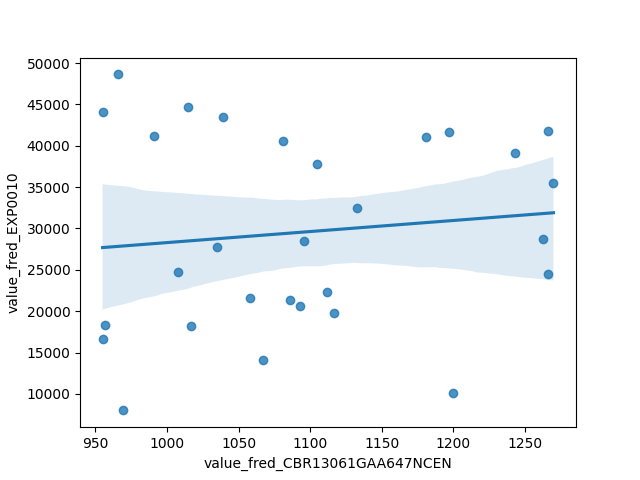
\includegraphics[scale = 0.9]{plots/plot_2025-01-14.png}
\caption{Regression Plot for 2025-01-14}
\end{figure}
\newpage

\section{Date: 2025-01-15}
\noindent \textbf{Series ID: COINDUSZ3332} 

\noindent This series is titled Import Price Index by Origin (NAICS): Industrial Machinery Manufacturing for Industrialized Countries and has a frequency of Monthly. The units are Index Jun 2012=100 and the seasonal adjustment is Not Seasonally Adjusted.The observation start date is 2012-06-01 and the observation end date is 2024-11-01.The popularity of this series is 1. \\ 

\noindent \textbf{Series ID: CUSR0000SERA02} 

\noindent This series is titled Consumer Price Index for All Urban Consumers: Cable, Satellite, and Live Streaming Television Service in U.S. City Average and has a frequency of Monthly. The units are Index Dec 1983=100 and the seasonal adjustment is Seasonally Adjusted.The observation start date is 1992-01-01 and the observation end date is 2024-12-01.The popularity of this series is 16. \\ 

\subsection{Regression Tables and Plots}
\begin{center}
\begin{tabular}{lclc}
\toprule
\textbf{Dep. Variable:}            & value\_fred\_CUSR0000SERA02 & \textbf{  R-squared:         } &     0.170   \\
\textbf{Model:}                    &             OLS             & \textbf{  Adj. R-squared:    } &     0.164   \\
\textbf{Method:}                   &        Least Squares        & \textbf{  F-statistic:       } &     30.23   \\
\textbf{Date:}                     &       Wed, 15 Jan 2025      & \textbf{  Prob (F-statistic):} &  1.64e-07   \\
\textbf{Time:}                     &           16:00:42          & \textbf{  Log-Likelihood:    } &   -809.02   \\
\textbf{No. Observations:}         &               150           & \textbf{  AIC:               } &     1622.   \\
\textbf{Df Residuals:}             &               148           & \textbf{  BIC:               } &     1628.   \\
\textbf{Df Model:}                 &                 1           & \textbf{                     } &             \\
\textbf{Covariance Type:}          &          nonrobust          & \textbf{                     } &             \\
\bottomrule
\end{tabular}
\begin{tabular}{lcccccc}
                                   & \textbf{coef} & \textbf{std err} & \textbf{t} & \textbf{P$> |$t$|$} & \textbf{[0.025} & \textbf{0.975]}  \\
\midrule
\textbf{const}                     &     -35.9024  &       93.848     &    -0.383  &         0.703        &     -221.357    &      149.552     \\
\textbf{value\_fred\_COINDUSZ3332} &       5.3316  &        0.970     &     5.498  &         0.000        &        3.415    &        7.248     \\
\bottomrule
\end{tabular}
\begin{tabular}{lclc}
\textbf{Omnibus:}       & 15.686 & \textbf{  Durbin-Watson:     } &    0.008  \\
\textbf{Prob(Omnibus):} &  0.000 & \textbf{  Jarque-Bera (JB):  } &   12.732  \\
\textbf{Skew:}          & -0.617 & \textbf{  Prob(JB):          } &  0.00172  \\
\textbf{Kurtosis:}      &  2.282 & \textbf{  Cond. No.          } & 2.08e+03  \\
\bottomrule
\end{tabular}
%\caption{OLS Regression Results}
\end{center}

Notes: \newline
 [1] Standard Errors assume that the covariance matrix of the errors is correctly specified. \newline
 [2] The condition number is large, 2.08e+03. This might indicate that there are \newline
 strong multicollinearity or other numerical problems.

\begin{figure}
\centering
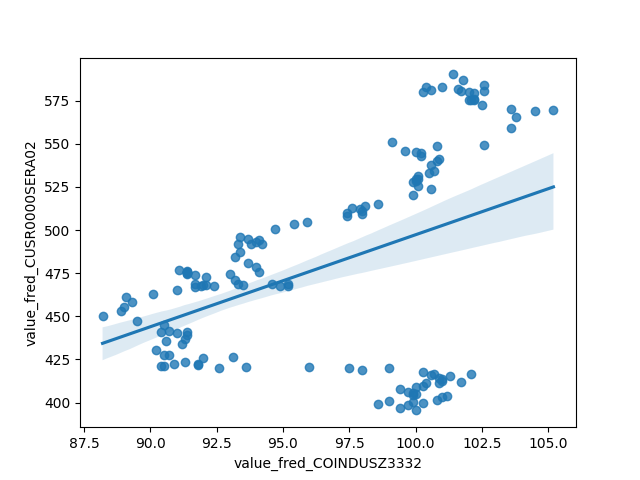
\includegraphics[scale = 0.9]{plots/plot_2025-01-15.png}
\caption{Regression Plot for 2025-01-15}
\end{figure}
\newpage

\section{Date: 2025-01-16}
\noindent \textbf{Series ID: ASMRMA} 

\noindent This series is titled All Sectors; Multifamily Residential Mortgages; Asset, Level and has a frequency of Quarterly. The units are Millions of Dollars and the seasonal adjustment is Not Seasonally Adjusted.The observation start date is 1945-10-01 and the observation end date is 2024-07-01.The popularity of this series is 33. \\ 

\noindent \textbf{Series ID: LRHU24MAJPA156N} 

\noindent This series is titled Infra-Annual Labor Statistics: Monthly Unemployment Rate Male: From 15 to 24 Years for Japan and has a frequency of Annual. The units are Percent and the seasonal adjustment is Not Seasonally Adjusted.The observation start date is 1968-01-01 and the observation end date is 2023-01-01.The popularity of this series is 0. \\ 

\subsection{Regression Tables and Plots}
\begin{center}
\begin{tabular}{lclc}
\toprule
\textbf{Dep. Variable:}      & value\_fred\_LRHU24MAJPA156N & \textbf{  R-squared:         } &     0.046   \\
\textbf{Model:}              &             OLS              & \textbf{  Adj. R-squared:    } &     0.029   \\
\textbf{Method:}             &        Least Squares         & \textbf{  F-statistic:       } &     2.615   \\
\textbf{Date:}               &       Thu, 16 Jan 2025       & \textbf{  Prob (F-statistic):} &    0.112    \\
\textbf{Time:}               &           11:42:02           & \textbf{  Log-Likelihood:    } &   -133.27   \\
\textbf{No. Observations:}   &                56            & \textbf{  AIC:               } &     270.5   \\
\textbf{Df Residuals:}       &                54            & \textbf{  BIC:               } &     274.6   \\
\textbf{Df Model:}           &                 1            & \textbf{                     } &             \\
\textbf{Covariance Type:}    &          nonrobust           & \textbf{                     } &             \\
\bottomrule
\end{tabular}
\begin{tabular}{lcccccc}
                             & \textbf{coef} & \textbf{std err} & \textbf{t} & \textbf{P$> |$t$|$} & \textbf{[0.025} & \textbf{0.975]}  \\
\midrule
\textbf{const}               &       5.3258  &        0.511     &    10.432  &         0.000        &        4.302    &        6.349     \\
\textbf{value\_fred\_ASMRMA} &    1.093e-06  &     6.76e-07     &     1.617  &         0.112        &    -2.62e-07    &     2.45e-06     \\
\bottomrule
\end{tabular}
\begin{tabular}{lclc}
\textbf{Omnibus:}       &  6.077 & \textbf{  Durbin-Watson:     } &    0.070  \\
\textbf{Prob(Omnibus):} &  0.048 & \textbf{  Jarque-Bera (JB):  } &    5.092  \\
\textbf{Skew:}          &  0.639 & \textbf{  Prob(JB):          } &   0.0784  \\
\textbf{Kurtosis:}      &  2.259 & \textbf{  Cond. No.          } & 1.08e+06  \\
\bottomrule
\end{tabular}
%\caption{OLS Regression Results}
\end{center}

Notes: \newline
 [1] Standard Errors assume that the covariance matrix of the errors is correctly specified. \newline
 [2] The condition number is large, 1.08e+06. This might indicate that there are \newline
 strong multicollinearity or other numerical problems.

\begin{figure}
\centering
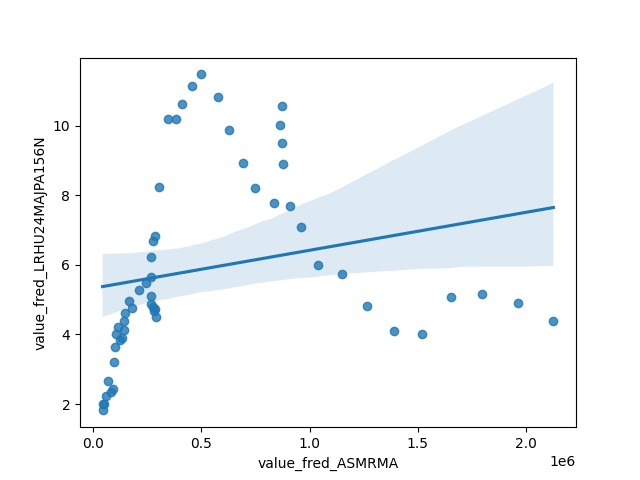
\includegraphics[scale = 0.9]{plots/plot_2025-01-16.png}
\caption{Regression Plot for 2025-01-16}
\end{figure}
\newpage

\include{tex_things/day_2025-01-17}
\include{tex_things/day_2025-01-18}
\include{tex_things/day_2025-01-19}
\include{tex_things/day_2025-01-20}

\end{document}
